\begin{wrapfigure}{r}{0.4\textwidth}
	\centering
	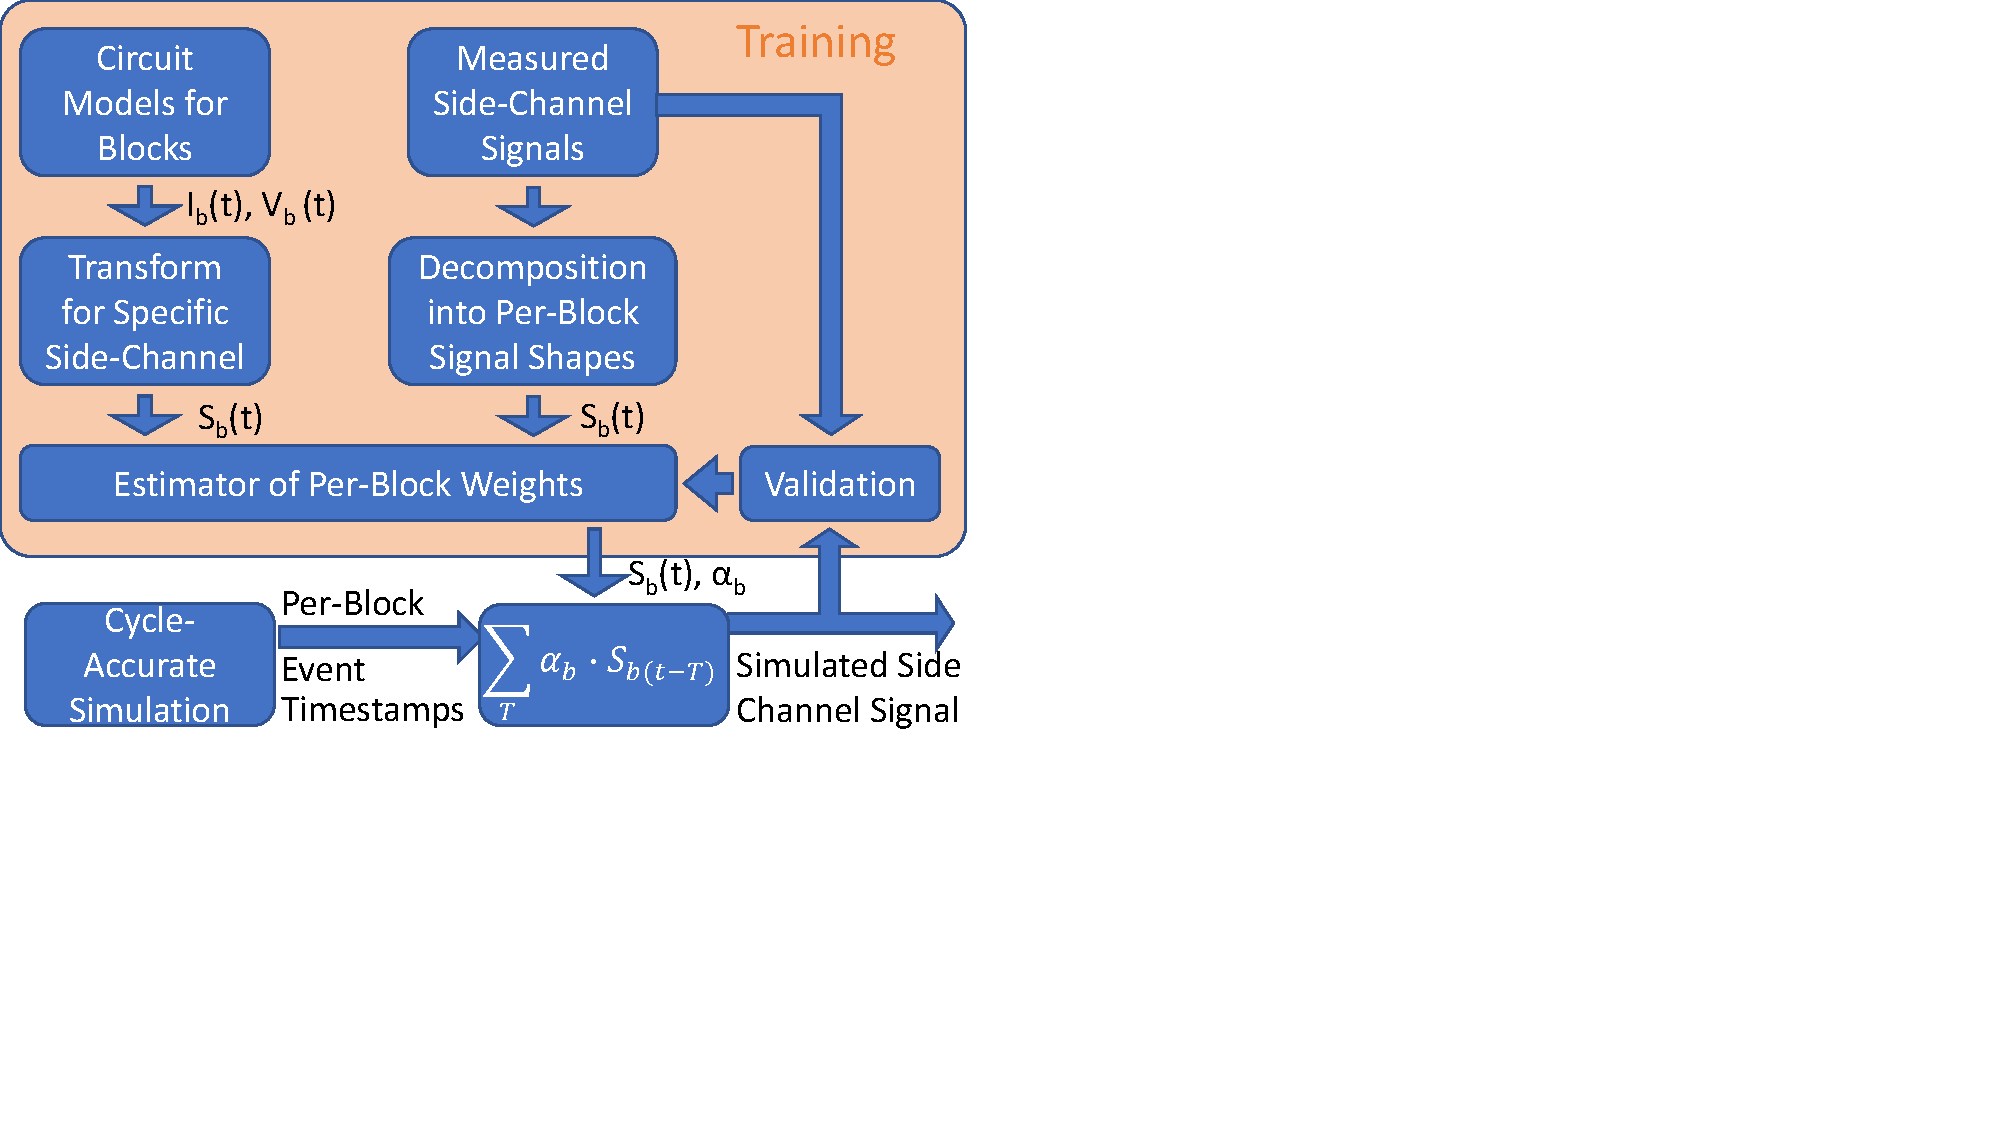
\includegraphics[width=0.4\columnwidth,trim={0in 2.65in 6.89in 0in},clip]{figure/overview.pdf}
	\caption{Overview of the proposed method.}
	\label{fig:overview}
\end{wrapfigure}

Figure~\ref{fig:overview} shows our overall proposed simulation approach. Most parts of this approach are within the orange-background ``Training'' oval in Figure~\ref{fig:overview}, which indicates that they are only needed for training, before the cycle-accurate simulation that constructs the overall simulated side channel signal begins. We propose to implement this overall signal construction efficiently by first preparing signal snippets for each type of event in each of the microarchitectural buling blocks within the processor, along with per-building-block weights that specify how to scale the contribution of each block when combining it into the overall side channle signal. Given these snippets and weights, we can obtain timestamps of individual events through cycle-accurate simulation and construct the overall signal by adding the appropriate snippet to the signal at each point in the signal's timeline where the corresponding event occurs. Our training (the ``Training'' oval in Figure~\ref{fig:overview}) constructs the signal snippets and their estimates weights through circuit-level simulation of individual events in individual building blocks, through decomposition of measured signals from an actual processor, or through a combination of these methods. Finally, simulation-generated signal can be calidated against measured signals and, if callibration agains that real processor is desired, discrepancies found during validation can be used to improve the snippets and weights in order to bring the future simulated results into better agreement with the measured signals.

To implement this approach, our proposed research consists of four primary research thrusts:

\begin{enumerate}
\item Finding how to efficiently generate detailed event timestaps and use them to combine signal snippets into the overall side channel signal, along with per-block and per-code-region breakdowns and attribution to help computer architects and software developers assess the impacts of microarchitectural and software changes on the tradeoff between performance, power, and side channel leakage.
\item Finding how to efficiently perform circuit-level simulation of caches, functional units, and other building blocks of the processor, to provide per-event timelines for voltage, current, and possibly other metrics that are needed to construct signal snippets for various side channels. along with other useful information such as how much the values of the metrics depend on data values.
\item Finding methods that produce per-event signal snippets for varous side channels, by 1) transforming the outputs of circuit-level simulation, 2) decomposing measured signals, or 3) synergistically combining both methods, and methods that estimate per-block weights.
\item Developing methods to validate simulated signals against measurements, and to adjust weights, signal snippets, and the simulator's timing parameters to calibrate snippets, weights, and timing parameters to a real processor.
\end{enumerate}

In the rest of this section, we provide more detail on each of these research thrusts, along with preliminary results that demonstrate the feasibility of the proposed approaches and provide an excellent starting point for the proposed research in each thrust.

\subsection{Thrust 1: Construction of Side-Channel Signals Through Cycle-Accurate Simulation}

With the scaled per-event signal snippets $S_b(t) , \dot \alpha_b$ from training, we can construct the side channel signal that corresponds to longer-term program execution. This signal construction uses a microarchitecture-level cycle-accurate simulation to determine the times at which each event occurr in each of the processor's block-level parts (ALU, decoder, reservation stations, cache, etc.), and these per-block event timestamps are then used to combine per-event signal snippets into an overall simulated signal. If validation against a real processor is desired, the simulation-generate and measured side channel signals can be compared, and the results of this comparison can be used to improve the estimation of per-block weights, or even (not shown in Figure~\ref{fig:overview})  to choose another circuit-level model that better matches the actual hardware of the processor.

One of the key research problems for this thrust will be to identify the tradeoff between the accuracy of the generated signal and the level of detai in the cyle-accurate simulation. Less detail, e.g. for an L1 data cache we may lump all events (hit, lookup with miss, fill following a miss) into a single ``cache action''  category that is represented by a single snippet. This would still allow the generated signal to capture the impact of the everall timeline of cache activity, e.g. having more prominent signals when executing code code regions with a lot of cache accesses, having low-signal-activity periods when the cache is not used (due to a processor stall between a miss and the corresponding fill), etc. However, these events would need to be differentiated to account for differnces between reads and writes, for lookups with a miss having to initiate an access in the next-level cache while hits to not, for fills writing an entire line while a write hit writes only a small part of the line, etc.

A similar tradeoff will be explored with respect to the impact of data values. We will start with data-value-agnostic simulation, which can still account for e.g. attackers being able to determine which part of the code is being executed, e.g. due to secret-dependent control flow. We will then add ability to obtain data-value statistics in cycle-accurate simulation,
and leverage the signal envelopes produced by our symbolic circuit-level simulation, to identify events (and blocks) whose signal snippets are the most affected by data values. For such blocks/events we will identify the nature of data-value dependency and construct data-value-dependent snippets, stansformations, and weights to account for data-value dependencies in the signal. We will do this selectively (not for all events) because there is a tradeoff between accuracy and training/simulation time, so a given amoung of accuracy improvement will come at a lower cost in training/simulation time is only the most data-value-dependent signal snippets are refined in this way.

\subsubsection{Preliminary Results for Thrust 1}

Our preliminary results for this thrust are based on EMSim~\cite{Nader2020}, a first-of-its-kind cycle-accurate simulator that generates practically relevant EM side channel signals for program execution on a canonical 5-stage pipelined processor. This simulator,
implemented by PI Prvulovic, Co-PI Zajic, and several PhD students they have co-advised, demonstrates the feasibility of using event timings from microarchitectural simulation together with signals snippets to generate overall side channel signals.

In EMSim, each pipeline stage of the processor is modeled as a single block, and each instruction is treated as a separate event for each stage. The signal snippets all use the same shape, which is a mathematical function. The results we show here use an sinusoid with rapidly declining (exponential) magnitude as the snippet shape. However, different events use snippet amplitudes (i.e. scaling factors), which are estimated using linear regression from signals that are measured on an FPGA-based impementation of this processor. Note that, although a more detailed RTL model of this processer was available,
we only used the microarchitectural model in our simulation, while the RTL was only used to actually implement the processor, and the scaling factors are then empirically obtained by running microbenchmarks on that real processor, measuring signals, and using linear regression to determine the  scaling factors that result in the best fit between the simulated and measured signals for those microbenchmarks..

\begin{wrapfigure}{l}{0.4\textwidth}
	\centering
	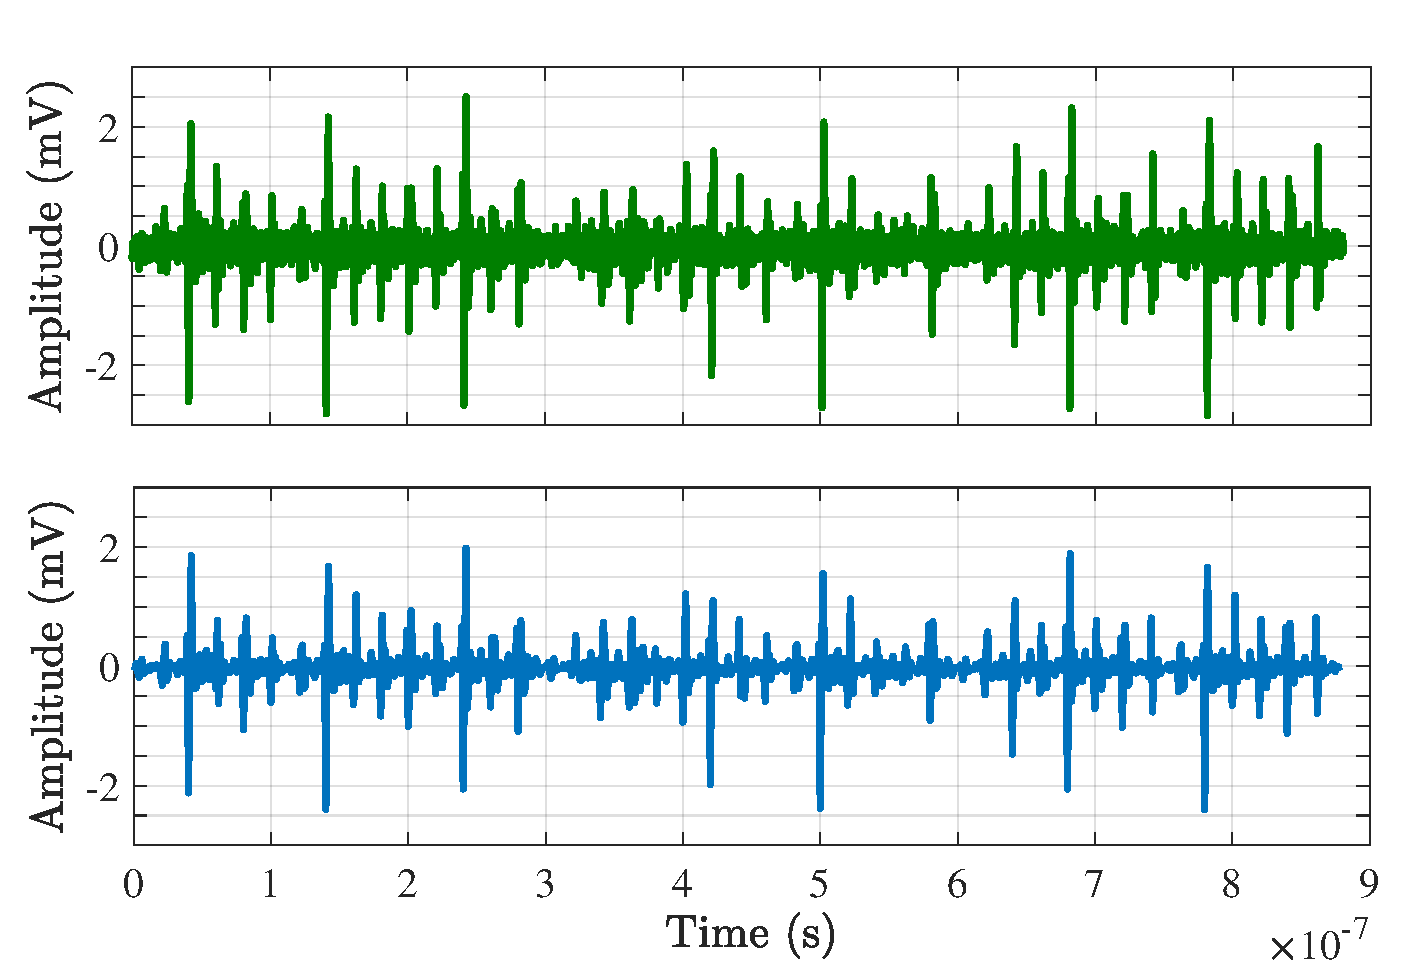
\includegraphics[width=0.4\columnwidth,clip]{figure/bench.pdf}
	\caption{A comparison between the signal generated by a real hardware (top) and the simulated signal (bottom) in EMSim.}
	\label{fig:bench}
\end{wrapfigure}
The scaled snippets are then combined into the overall simulated side channel signal for previously unseen program code (not used to obtain scaling factor). For this, we use a microarchitecture-level simulator to model the pipeline of the processor. In each cycle,
for each stage of the processor this simulator identifies which instruction is in that stage in that cycle, i.e. which event occurs in each of the ``building blocks'' of the processor, and
the ``snippet'' with the block-and-event-dependent magnitude is added to the overall signal at that point in time. The resulting signal for one such simulation is the bottom signal in Figure~\ref{fig:bench}, while a measured signal for the same program sun (same code and data values) is shown above it (also in Figure~\ref{fig:bench}). We observe that, alstohugh the signals have some differences, most of the prominent features from the measured signal are also present in the simulator-generated signal.

In the same work (EMSim~\cite{Nader2020}), we have also demonstrated the importace of modeling timing and microarchitectural behaviors, i.e. the need for using a cycle-accurate simulation of the microarchitecure rather than a simpler emulator of the instruction stream.

\begin{wrapfigure}{r}{0.4\textwidth}
	\centering
	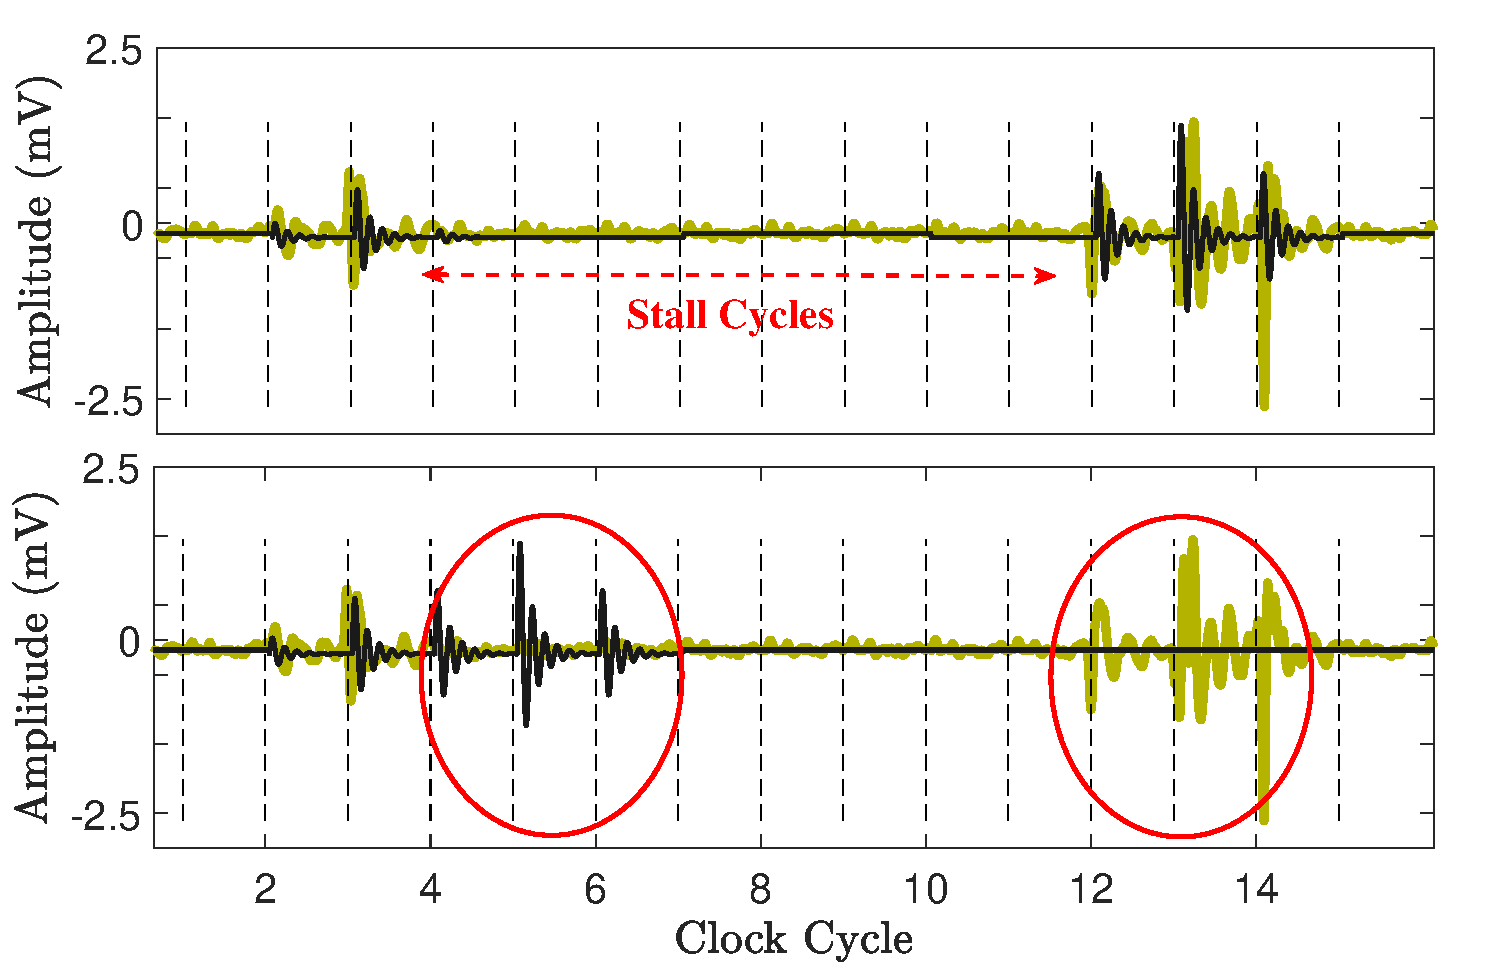
\includegraphics[width=0.4\columnwidth,clip]{figure/stall2.pdf}
	\caption{Effect of stalls on the signal. The actual signal shown in green, while simulated signals are shown in black when modeling pipeline stalls (top) and not modeling it (bottom).}
	\label{fig:stall}
\end{wrapfigure}
To illustrate the need to account for microarchtectural events, in Figure!\ref{fig:stall} we show the effect of a pipeline stall (for clarity, we cause a stall by increasing the latency of a MUL instruction to eight cycles, where the next instruction uses the result of that MUL) on the signal's timeline. The top part in Figure~\ref{fig:stall} is the simulated signal that models the pipeline stall, along with the measured signal for the same part of the program execution. However, it pipeline stalls are not accounted for (in this case, by ignoring the effects of the dependence between the MUL and the next instruction), the timeline of the simulated signal changes significantly (bottom part of Figure~\ref{fig:stall}) and has no longer has an excellent match to the measured signal. Similar effects are observed when the simulation ignores other microarchitectural events and their timing, e.g. if caches are not modeled (all load/store treated as hits), if branch prediction is not modeled (no branch mispredictions), etc.

\begin{wrapfigure}{l}{0.4\textwidth}
	\centering
	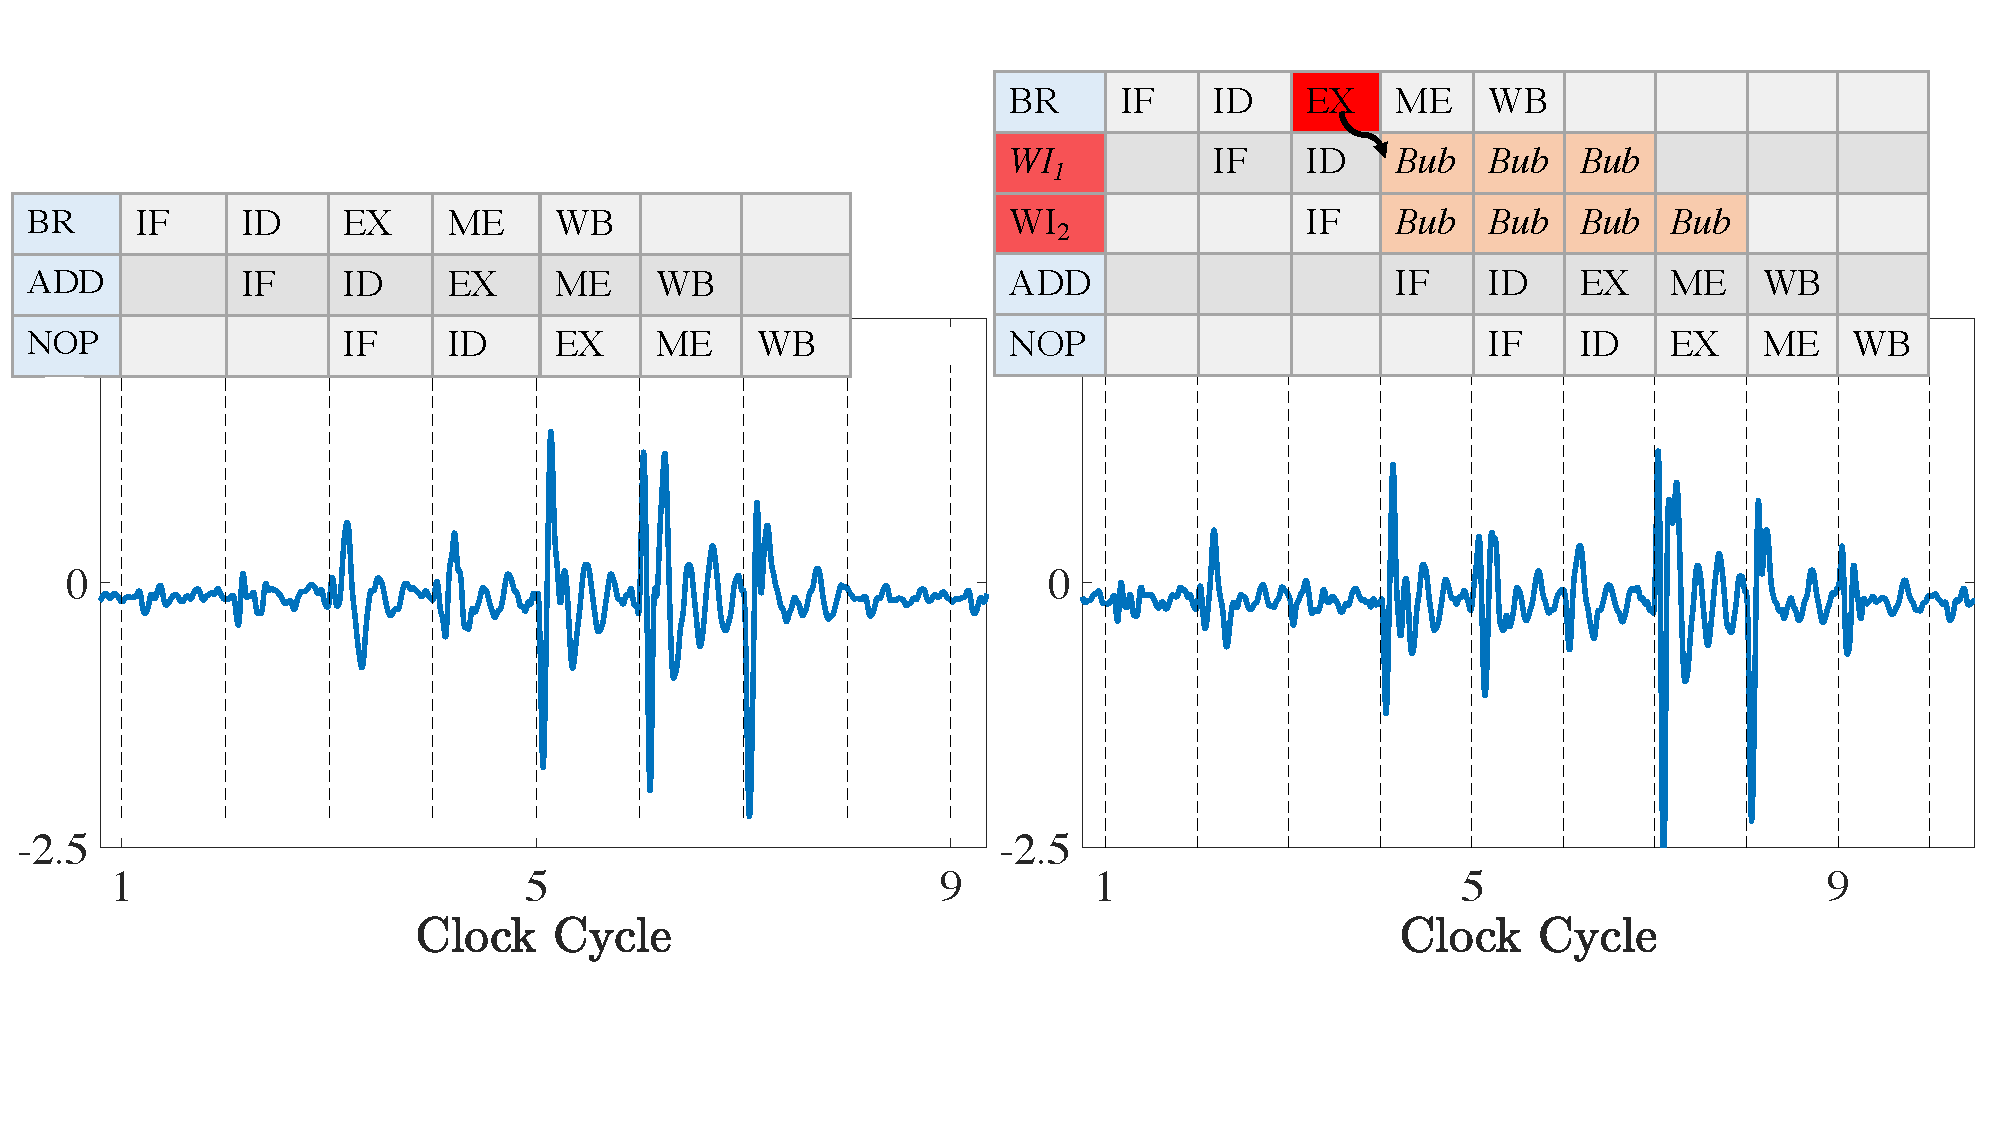
\includegraphics[width=0.4\columnwidth,clip]{figure/mise2.pdf}
	\caption{Effect of misprediction (right) on the signal. It causes two instructions being flushed from the pipeline and hence affect the signal in those cycles.}
	\label{fig:mis}
\end{wrapfigure}
In addition to its impact on timing, we observed that a branch misprediction also has noticeable impact on the shape of the side-channel signal. In the 5-stage processor that was used in EMSim, a branch misprediction causes a flush of the first two pipeline stages, which not only adds two cycles to the execution but also changes which instructions are in which stage of the pipeline for the next few cycles, as shown in Figure~\ref{fig:mis} with real (measured) signals. Therefore, if the simulated signal is put together without modeling branch prediction (and accounting for mispredictions), the signal differs significantly. This effect would be even more pronounced for a more sophisticated processor (more instructions flushed and more change in overlap among activity in different stages/blocks).

Overall, even though EMSim had used the a simple mathematical function as the snippet shape for all events, the side channel signal it constructs matches the measured EM side channel signal relatively well. To evaluate EMSim, we had used programs that were specifically generated to create various combinations of instructions in different pipeline stages, resulting in 34 programs that execute for about 9,000 cycles each. We used \textit{normalized cross-correlation} as our accuracy metric.

Overall, we found that EMSim achieves 94.1\% accuracy in simulating the EM side-channel signals. While this is sufficient for many purposes, e.g. assessing vulnerability to simple power attacks (SPA) and simple EM attacks (SEMA) that extract secrets by differentiating between executing different parts of the program code (e.g. a secret-dependent if-then-else) and/or differential attacks (DPA, DEMA) that depend on large differences in values that are operated on, more accuracy is likely to be needed for simulated signals to be used to assess vulnerability to more sophisticated attacks that differentiate between data values that are similar to each other. We expect that the proposed use of per-event signal snippets from circuit-level simulation, with additional data-value-dependent considerations, will enable such uses of our simulation-generated signals. Additionally, our proposed work will enable signals to be generated not only for the (simplest) pipelined processors, but also to the much mode complex processors (deep pipelines, superscalar, out-of-order, etc.), by extending cycle-accurate simulators such as GEM5~\cite{gem5}.

\subsection{Thrust 2: Construction of Per-Event Current/Voltage Timelines via Circuit-Level Simulation}

Even when a full circuit-level model for an entire processor is available, circuit-level simulation is not efficient enough to go through numerous program runs, with billions of processor cycles in each run, that would be needed to provide computer architects and software developers with actionable insights about the impact of microarchitectural and/or software changes on the tradeoff between performance, energy, and side-channel vulnerability. For example, PI Kumar's symbolic execution framework~\cite{cherupalli2017} currently uses detailed gate-level models of the microprocessor hardware, resulting in high-fidelity reproduction of metrics that are needed to predict the microprocessor's EM and power side-channel signals, but this  at a high computational cost when modeling entire-program execution -- an FFT implementation for a 16-bit MSP430 DSP takes over 3 hours, and this time would become several times longer for more complex processors and orders of magnitude longer for realistic runs of larger applications.

Instead, our proposed approach raises the abstraction level of the whole-program simulation to the microarchitecture level (i.e. cycle-accurate simulation), and will use circuit-level simulation only during training, separately for each block of the processor, e.g. decoder, adder, multiplier, instruction scheduler, cache, etc. to produce, for each kind of activity in a block, how currents and voltages in that block change over time (i.e. $I_b(t)$ and $V_b(t)$) during that activity. Note that each of these circuit-level simulations is very brief, as it only needs to account for activity that corresponds to a single event (e.g. for a cache the events would be a lookup with a read-hit, lookup for a read-miss, fill on a read-miss, and read completion after a miss and fill, and the corresponding events for a write), so each of these circuit-level simulations models only a few processor cycles, albeit with a great level of detail.

To improve accuracy of our overall signals, we will leverage the ability of the existing circuit-level simulator to evaluate circuit activity for symbolic data.  As such, for a given time period, the current, voltage, etc. signals are each best modeled as a time-chaging distribution, or as an  ``envelope'' that shows the possible range of values at each point in in time, rather than a single curve. This presents us with a number of research challenges: how to express these distributions in the way that aids accuracy of the overall signals produced by cycle-accurate simulation, how to prevent path explosion when modeling blocks that may have significant changes in activity depending on the data (e.g. a symbolic address causing a hit or a miss in a cache), how to express aggregate data-dependent amounts as simplified symbolic expressions, to allow microarchitecture-level simulation to account for significant changes in aggregate activity within a block without resorting to modeling the block at a lower lever of abstraction, etc.

To help designers of highly secure microprocessors, i.e. processors which should have minimal information leakage via side-channels for {\tt any}program, we will also investigate a complementary approach, Property Driven Automatic Transformation (PDAT)~\cite{bleier21}, which analyzes net switching activity within a circuit for any inputs and performs model checking that allows processor designers to choose (or redesign) specific building blocks in a way that minimizes data-dependent changes in activity that would leak information. In essence, rather than accounting for data-dependent activity and expressing it in the signals provided to cycle-accurate simulation, this approach changes the hardware of the block to minimize such data-dependent activity, likely eliminating the need to account for data-dependent activity for that block.

Finally, while we expect that overall current and voltage will allow our side-channel-specific transformations to produce highly accurate signal snippets, more entailed outputs, e.g. separate $I_b(t)$ and $V_b(t)$ for different kinds of circuit elements, e.g. transistors, interconnect wires, power delivery wires, etc. may be needed to further improve accuracy, and we will investigate both the need for such refinements, and how to implement them efficiently. For example, transistors that have the same geometry may have similar impact on side-channel-relevant properties (current, voltage, etc.), and thus may be represented in aggregate, but activity of larger transistors may need to be aggregated separately from smaller ones, to allow different scaling factors to be used for their activity when generating side channel snippets and/or accounting for data-dependent changes in the side channel signal.

\subsubsection{Preliminary Results for Thrust 2}

\begin{wrapfigure}{l}{0.4\linewidth}
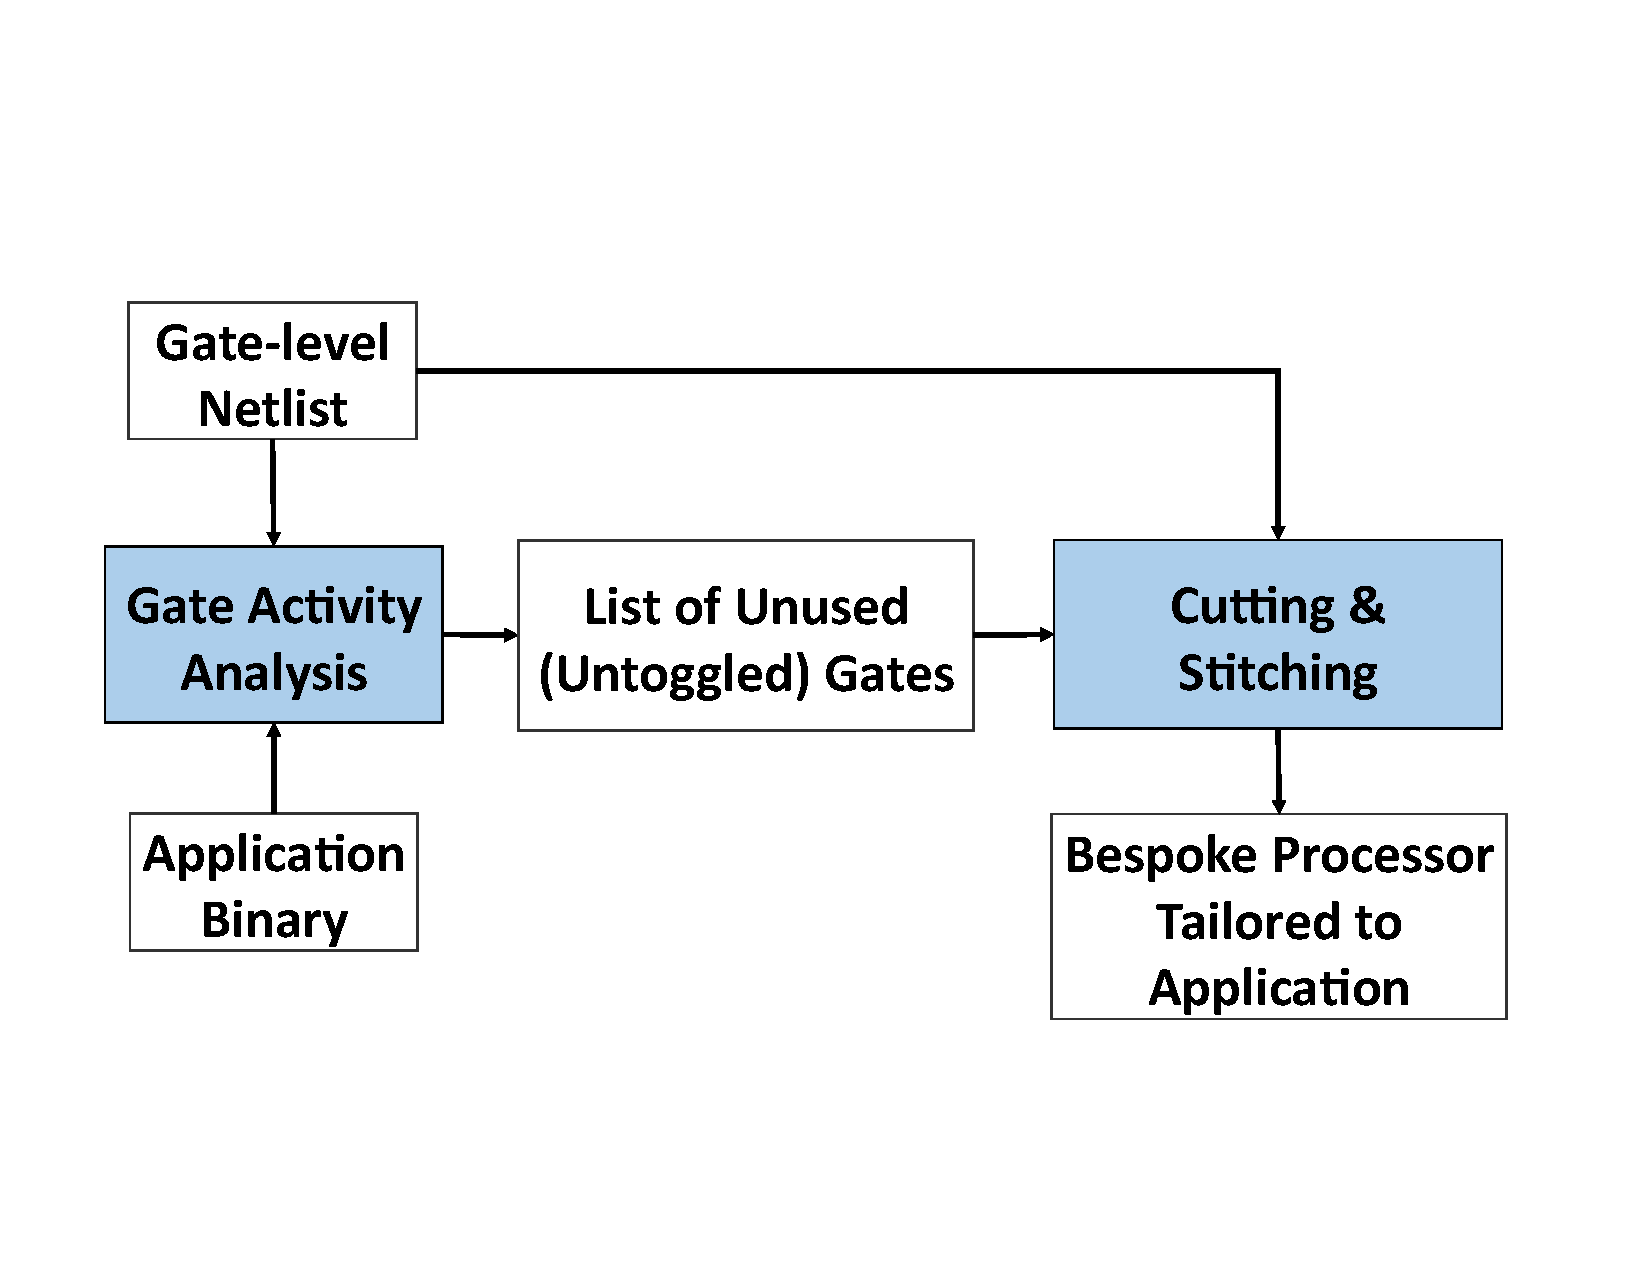
\includegraphics[width=\linewidth]{./figure/Bespoke_Flow_Fig.pdf}
\caption{\small
    Hardware-software co-analysis used to generate bespoke microprocessors.}
\label{fig:bespoke}
\end{wrapfigure}
Co-PI Kumar's prior efforts to enable software developer to analyze their software for analog side channels have resulted in a framework which performs symbolic execution of a program on a detailed (gate-level) model of a microprocessor~\cite{cherupalli2017}.
This framework was originally developed in order to automate design of `bespoke microprocessors' --- microprocessors designed to execute a single application binary.
The flowchart for this use case is in shown in Figure~\ref{fig:bespoke}, and the symbolic execution of the program on the hardware occurs in the `Gate Activity Analysis' stage.

This framework accounts for how activity within the processor is affected by program inputs (e.g. sensor inputs in an IoT system), both for data-dependent (data values) and instruction-dependent (which instructions end up being executed) activity within the circuitry of the processor. This symbolic execution framework can identify whether any possible execution of a program leads to significant changes in gate-level activity and, consequently, side-channel leakage, allowing programmers to to add or remove often-expensive software mitigation techniques depending on which mitigations are actually needed. This framework has shown applicability for security applications~\cite{cherupalli20172}, including
taint-tracking for information flow security to locate information policy
violations, even violations which result from covert timing side-channels.

This prior work provides us with an excellent starting point for the proposed symbolic circuit-level simulation. However, as pointed out earlier, circuit-level simulation of an entire processor throughout the execution of a program is exceedingly slow compared to state-of-the-art microarchitecture-level (cycle-accurate) simulation. Our proposed approach will synergistically combine the advantages of symbolic circuit-level simulation and microarchitecture-level simulation, using circuit-level simulation only duringtrainingto generate accurate per-event signal snippets, and using the (orders of magnitude faster) microarchitecture-level simulation to model the entire microprocessor for an entire program execution and generate a side channel signal by combining pre-made snippets.

Additionally, which gate-level switching activity can be a good proxy for side channel information leakage, PI Prvulovic and Co-PI Zajic's past work~\cite{Nader2020} has shown that the mapping from gate-level activity to side channel signals tends to be proportional only for gates within a relatively homogenous block (e.g. a cache, a multiplier, etc.), but the scaling factors for different blocks can differ significantly. Thus our proposed approach is to account for these unequal transformations on a block-by-block basis, accounting for the specifics of how each side channel (EM, power, etc.) is affected by gate-level events, to produce {\em side channel signals} (rather than proxy metrics) that can be compared to and callibrated against measured signals for varous side channels/

\subsection{Thrust 3: Per-Event Side Channel Snippet Construction and Scaling}
\label{sec:proposed-transform}

This research thrust will explore 1) how to transform the results of the circuit-level simulation into a signal snippet that represents the shape of the side channel signal that is contributed to the overall side channel signal by an occurrence of that event, 2) how to estimate the magnitude and (at least to some extent) the shape of these side channel signal snippets by decomposing measured signals, and 3) how to synergistically combine the side channel snippets obtained from circuit-level simulation and from signal decomposition.

Specifically, after the circuit-level simulator produces $I_b(t)$ and $V_b(t)$ signals for a specific event that happens in a specific block, we need to transformed this into side-channel signal snippet $S_b(t)$. This step accounts for the impact that current and voltage (and their changes over time) have on that side-channel. For example, for the power side channel the transformed signal would be the product of the current and voltage signals, for the EM side channel the transformed signals would be using Maxewell' equations to produce transformed signals that are proportional to the first derivative of the curent and voltage signals, etc.

Snippets $S_b(t)$ can also be obtained from measurements of side channel signals on a real processor. This is needed, for example, when a circuit-level model of some part of the processor is not available, or to correct (or calibrate) the scale of snippets from circuit-level simulations that have systematic biases, e.g. due to imprecisions in transistor models or lack of accounting for some electrical, electromagnetic, or quantum effects during circuit-level simulations. Our initial approach to obtaining per-event snippets from measured data will
be to collect side channel signals as the processor executes various microbenchmarks that are designed to create specific of events in specific parts of the processor, allowing the measured signals to be decomposed into signal snippets that correspond to contributions of individual events in individual units (e.g. using SVD).

Finally, we note that the two methods of obtaining per-event signal snippets are highly complementary. Specifically, because of measurements noise and bandwidth limitations, these measurement-derived snippets tend to be more accurate in terms of the overall contribution of the event to the signal (e.g. the average signal magnitude contributed by the event) over its ``life span'' (i.e. the few cycles during which the single occurrence of the event affects the signal), and less accurate in terms of the shape, i.e. change-over-time of the signal snippet during the event's ``life span''. Conversely, circuit-level models are likely to produce very accurate shapes -- if N identical-in-size transistors toggle, the current draw is proportional to N -- but the magnitude of these shapes may not be scaled correctly if the transistor parameters do not match the actual ones precisely. This means that, when both circuit-level models and empirical measurements are available, the model-generated signal snippets can be scaled to match the average magnitude of measurement-derived signals. This combining, along with other activities that involve scaling and callibration of simulated against measured side-channel signals, is part of the next research task.

As already noted in Section~\ref{sec:proposed-transform}, per-event snippets generated by from circuit-level simulations contain a lot of detail and metadata (e.g. the ``envelope'' for the signal that shows how much the signal snippet can change due to different data values), but may have systematic biases due to imperfect modeling of device physics, device parameters, or the circuit, and these biases are likely to mostly affect the scale of the snippet rather than its shape. Conversely, obtained by decomposing measured signals have much more accuracy in their overall magnitude (scale) than they have in their exact shape. To synergistically combine these methods, our initial approach will be to estimate the per-block scaling factors (weights) $\alpha_b$, and we will refine this as needed to improve accuracy further (e.g. using functions other than simple multiplication with a constant scaling factor).

The second reason for using weights (or other ``scaling'' functions) is to account for side-channel specific differences in attenuation of signals from different blocks. Specifically, for the EM side channel, the EM signal contribution from one block may experience more propagation loss than signals from another block, depending on the materials each signal propagates through and/or the position of the antenna or probe. These differences in propagation can also be accounted for using the per-block scaling factors $\alpha_b$, which can be determined using either measured signals or simulation-based propagation models.

Finally, we will account for data-dependent activity by accounting for how the signal is affected by values both between the microarchitecture-level builings blocks and within each block. Fundamentally, signals in most side channels (e.g. EM and power) are created during  \textit{bit-flips} at the transistor-level~\cite{VANECK1985269,6766222}, i.e. by changes in values at outputs of individual gates, flip-flops, and entire building blocks. Values that are outputs of individual blocks (e.g. the result produced by an ALU or the value read from a data cache) are typically already tracked during cycle-accurate simulation, so we can account for how changes in these values affect the side channel by adjusting the scaling factors according to data-dependent metrics such as the number of bit-flips. Values within a building block (e.g. values of carry bits within an adder or values produced by individual stages within a multiplier), however, are typically not tracked by a cycle-accurate simulator, and doing so precisely would be very costly in terms of simulation time. However, we note that values at outputs of building blocks tend to drive long interconnect wiring, whereas the wiring that carries values within a block tends to be local. This implies that for most analog side channels, e.g. power, EM, etc., values at outputs of building blocks will tend to have a significantly stronger impact of the overall side channel signal, and this is also supported by our preliminary results. Therefore, bit-flips within a building blocks are likely to have an aggregate effect, i.e. the side channel signal is affected mostly when data values at inputs of the block produce large differences in the amount of internal bit-toggling. Rather than add simulation of such intra-block activity to the cycle-accurate simulator, we plan to account for this in the aggregate, by leveraging the ability of our circuit-level simulators to consider symbolic outputs and produce the envelope that describes how much the signal can vary depending on input values and, if such signal variation is significant enough, by generating symbolic expressions for how the aggregate amounts of internal switching depends on the input values of the block.

\subsubsection{Preliminary Results for Thrust 3}
\label{sec:prelim-transform}

Our preliminary results for this thrust are also based on our work on EMSim~\cite{Nader2020}, where we considered two main contributors to the EM side-channel signal contributed by each building block (in EMSim, an entire pipeline stage of the simple 5-stage pipelined processor is treated as a building block). The first group of contributors, which we call \textit{instruction-dependent} contributors, consists of per-use signal contribution of each micro-architectural block, e.g. whether instruction fetch is happening or not (due to a stall) in a particular cycle, whether the register-file is being written in the last stage of the pipeline or not in a particular cycle, etc.

The second group of contributors is \textit{data-dependent} activity, which is created by bit-flips on the long wires, such as address and data lines going to/from the cache, and in registers that hold values of operands. In reality, operand and data values also change the signal in other parts of the processor, e.g. on wiring between gates within an ALU, but for EMSim we only accounted for address, data, and operand values because those are already available during cycle-accurate simulation, whereas accounting for other bit-flips would have required TRL-level or circuit-level modeling (which was not done for EMSim).

For both types of contributors, we assumed that activity creates a signal that has the same overall shape (an exponentially-decaying sinusoid), because we did not use circuit-level models to get a better estimate of the shape. However, the magnitude of that shape is estimated separately,using measured data, for each contributor. For instruction-dependent contributors, i.e. effect on the signal of a specific type of instruction utilizing a specific pipeline stage, this estimation relies on executing microbenchmarks in which a single instruction, surrounded by NOP instructions, is executed, with all of its operands and data values set to zero, to minimize the effect of data-dependent contributors and create a {\tt baseline} level of activity for each type of instruction in each stage of the processor.

\begin{wrapfigure}{l}{0.4\textwidth}
	\centering
	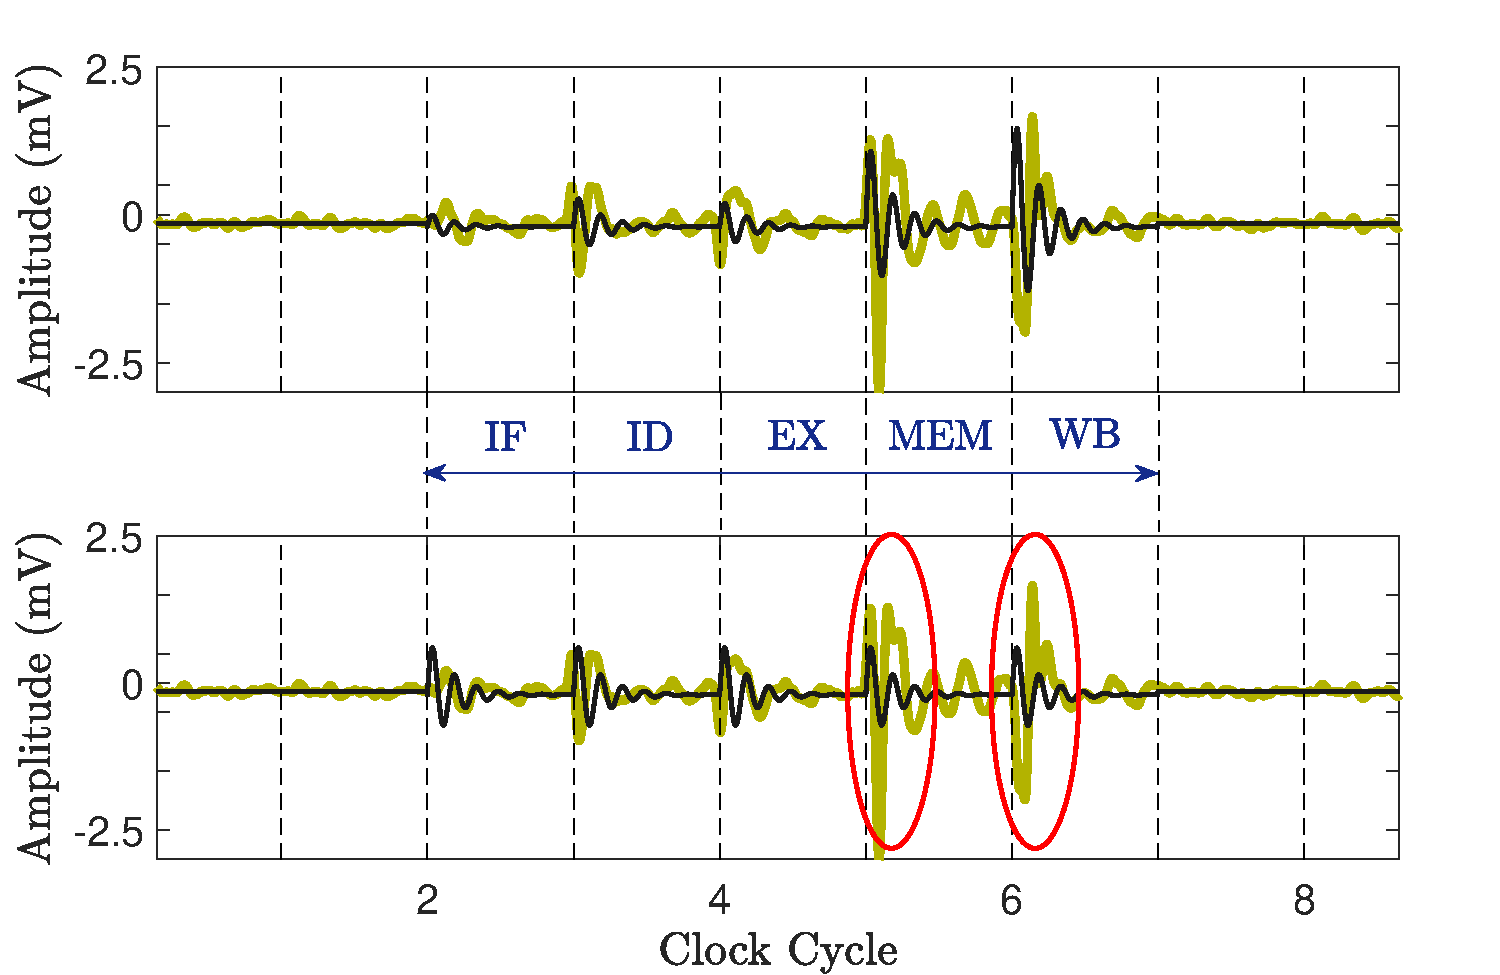
\includegraphics[width=0.4\columnwidth,clip]{figure/amp2.pdf}
	\caption{The signal amplitude for an {\tt ADD} as it progress in the pipeline (while all other instructions are {\tt NOP}). The actual signal is shown in light color (green). Darker color (black) shows the simulated signal when considering each pipeline stage as a separate source (top), and when considering the entire processor as a single source (bottom), and the largest differences between the two are pointed out using red ellipses.}
	\label{fig:amp}
	\vspace{-5mm}
\end{wrapfigure}
Figure~\ref{fig:amp} shows how the measured EM signal (shown in green/light color in both parts of this figure) changes as an {\tt ADD} instruction progresses through the pipeline while all the other instructions are {\tt NOP}s.
%Using Equ.~\ref{equ:em} \cite{Nader2020} and {\tt NOP}$\rightarrow$ {\tt inst}$\rightarrow$ {\tt NOP} instruction sequence, we used our simulator to generate the signal.
%\begin{equation}
%y(t) = \sum_{n=0}^{+\infty} x[n] \sin(\frac{2\pi(t-nT)}{T_0})  e^{-\theta(t-nT)}  \mathtt{u}(t-nT).
%\label{equ:em}
%\end{equation}
%This equation represents two main effects we observed in the analog side-channel signal: 1)
%\textit{switching activity in a processor is synchronized to its clock} and most of the switching happens right after the positive/negative edge of the clock, which implies that activity is not evenly spread over a cycle and a decaying function can be used to model clock activities; 2) \textit{the received signal is also exposed to oscillations with decreasing magnitude}, i.e., small signal variations can be modeled as sinusoidal oscillations.
The top part of Figure~\ref{fig:amp} also shows the corresponding simulated signal, where the contribution of each stage is modeled as an exponentially-decaying sinusoid snippet, each scaled using the magnitude obtained from measured data. To show why individual stages should be modeled separately, the bottom part of Figure~\ref{fig:amp} shows the simulated signal when all stages are treated as being the same, i.e. only one (average) amplitude is estimated from measurements and used for activity in any stage. As can be seen, failing to model each stage individually (as used in previous work~\cite{McCann:2017:TPT:3241189.3241207}) can lead to significant inaccuracies for most stages.

For data-dependent contributors, the pipeline simulator used in EMSim identifies the number of bit-flips on address and data lines and in the register being written. Intuitively, more bit-flips cause more current flow and thus larger amplitude of EM emanations. To combine the effects of such data-dependent activity with the baseline (instruction-dependent) activity, we define the \textit{activity-factor}, $\alpha$, as a \textbf{\textit{scaling factor}} for each baseline activity $A$. To find this $\alpha$, we assume all bit-flips within the stage contribute equally, i.e. that each bit-flip contributes equally to the signal amplitude. Becasue the baseline signal amplitude already includes some bit-flips (e.g. becasue instruction addresses and instructions themselves are non-zero when accessing the instruction cache, we calculate $\alpha$ as $\alpha = 1 + \frac{(\mathit{flips}_{new} - \mathit{flips}_{base})}{\mathit{flips}_{total}}$, where $\mathit{flips}_{new}$ is the total number of flips for the current instruction,  $\mathit{flips}_{base}$ is the total number of flips when previous instruction is {\tt NOP}, and $\mathit{flips}_{total}$ is the maximum possible number of flips for the current instruction. The overall scaling factor for the (decaying sinusoid) snippet is then $A' = \alpha\times A$.

\begin{wrapfigure}{l}{0.4\textwidth}
	\centering
	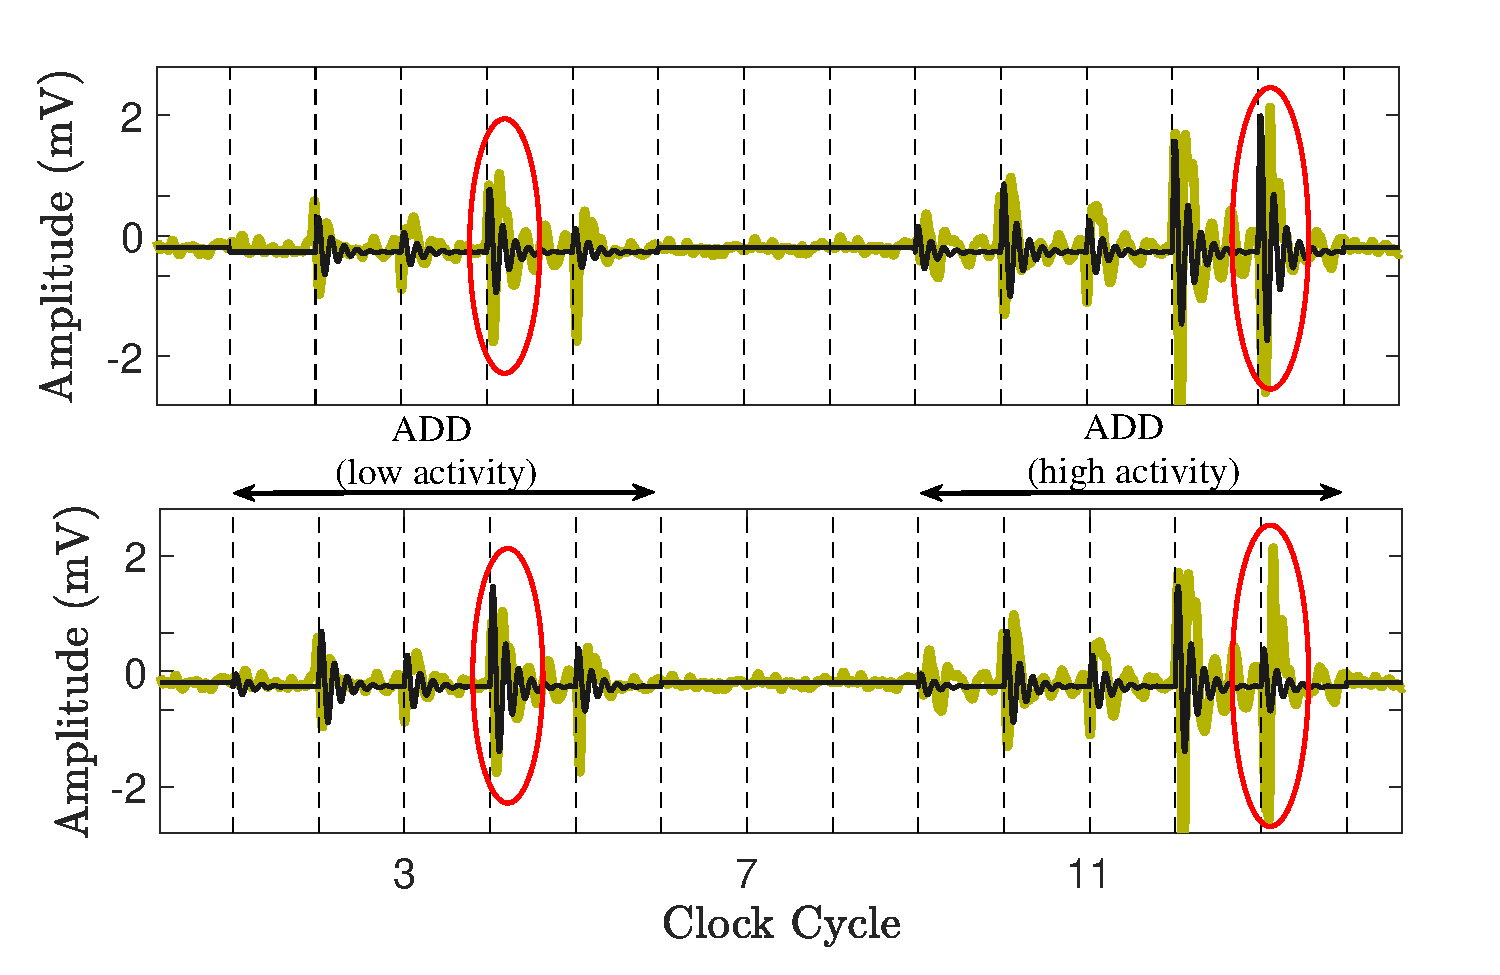
\includegraphics[width=0.4\columnwidth]{figure/alpha2.pdf}
	\caption{Effect of the \textit{activity factor} on the amplitude. The actual signal shown in green. The simulation is shown in black when activity factor is modeled using a linear regression model (top) and when an \textit{average} activity is used (bottom).}
	\label{fig:alpha}
\end{wrapfigure}
To illustrate why these data-dependent considerations need to be accounted separately for each block, Figure~\ref{fig:alpha} shows the measured signal as green/weak and the simulated signal as black, where the simulated signal in the top part uses per-stage activity factors in each cycle as described above, while in the botom part the simulation always uses one (average) activity factor. We observe that accounting for data-dependent activity in at lest some parts ofthe processor is needed to achieve good accuracy of the simulated signal. Further analysis of measured data has also shown that not all bit-flips have the same effect on the signal. Specifically, we found that 1) bit-flips in the output of the ALU and the cache have the most significant impacts on the signal, which can be expected in this FPGA-based design because these outputs were the driving the longest total amount of interconnect to reach all of their fanout targets, and 2) bit-flips in about 64\% of block output bits had a negligible contribution to overall accuracy (as determined through stepwise regression~\cite{f-test}). This supports our proposed approach of using measured data to estimate the contribution of each block (and how much of it is data-dependent), and then selectively add accounting for data-dependent activity only for blocks where such accounting can result in a meaningful improvement in accuracy. Also, our preliminary findings are encouraging because the largest data-dependent contributions were outputs of entire units (ALU, cache, etc.) rather than internal wiring within these units, i.e. the most impactful bit-flips occur in values that are already modeled by cycle-acurate simulators, while the values on wires within an individual block have less of an effect. However, in our proposed work we plan to use aggregate accounting for toggling within blocks through symbolic circuit-level simulation to obtain not only the ``baseline'' signal snippets for each block, but also the input-dependent expressions for how the shape of the signal snippet would be affected by the values at the block's inputs and, for register files, caches, etc., by changes to values stored within those blocks.

\subsection{Valiidation/Callibration Aginst Measured Signals}

In this thrust we will evaluate the accuracy of snippet generation, transformation, and overall simulated signals produced by the methods we develop, using measured side channel signals collected from real processors. The results of this evaluation will help us identify likely sources of error and refine our methods, which will allow us to refine our approach to create efficient simulators that produce highly accurate side channel signals that are callibrated against specific real processors.

The insights from this evaluation, refinement, and calibration efforts will hen be used to design systematic mechanisms that can automate this iterative refinement/callibration, resulting in mechanisms that selectively refine the circuit-level models, accounting for data-dependent behaviors, scaling factors, and other aspects of the training process to achieve a desired level of accuracy while minimizing the impact of these refinements on simulation time and avoiding costly refinements (e.g. development of more detailed circuit-level models) that would not result in a commensurate increase in accuracy of the simulated signals.

\subsubsection{Preliminary Results for Thrust 4}

Co-PI Kumar in experienced in digital design, chip design,
tape-out, and testing, and runs an undergraudate course in which students design processors that are then are manufactured by TSMC and tested on the UIUC campus.
His group has also participated in Intel's Chip Design Challenge, manufacturing RISC-V microprocessors in Intel's 16 nm technology. This gives us a sizeable collection of microprocessor artifacts, with both large and small microarchitectural differences,
which can be subjected to side-channel measurement and also modeled at various levels of abstraction -- high-level microarchitecture, RTL, gate-level,
GDS/geometry level, and physical chips. This will allows us to evaluate the predictive accuracy of the simulation-generated signals with respect to microarchitectural changes,
and also to calibrate based on numerous real-world designs and implementations.

PI PRvulovic and Co-PI Zajic have extensive experience in side-channel measurements for EM, power, and several other analog side channels (acoustic, optical, temperature, ...), comparing these signals to each other, and, more recently, comparing synthesized or modeled signals to measured ones~\cite{Nader2020} and using the results of these measurements to refine the models. 